\documentclass[12pt,a4paper]{article}
\usepackage{minted}
\usepackage[brazil]{babel}
\usepackage[utf8]{inputenc}
\usepackage{graphicx}
\graphicspath{ {./img/} }
\usepackage{amsmath}



\title{Relatório Prática 1}
\author{Vitor Barbosa}
\date{\today}
\begin{document}
\maketitle
\section{Introdução}
Nesta prática, faremos o bom e velho Hello World em C++. 

Sempre que necessário, utilizarei o Qt na resolução dos exercícios por ser uma ferramenta multiplataforma madura para a criação 
de interfaces de usuário. 

O Qt suporta Windows, Mac, Linux, Android e até mesmo dispositivos embarcados(na versão comercial).

Ele está disponível sob as licenças LGPL e GPL para aplicações de código aberto.
\section{Código}
Arquivo \emph{main.cpp}
\begin{minted}{cpp}
#include <QApplication>
#include<QWidget>
#include <QLabel>

class Hello:public QWidget{
public:
//Construtor
    Hello(QWidget *parent = 0):QWidget(parent){
        // Cria um QLabel com o texto Hello World
        QLabel *label  = new QLabel("Hello World!",this);
        //Tamanho do QLabel
        label->setGeometry(75,50,100,50);
    }

};

int main(int argc, char *argv[])
{
    //Precisamos criar um QApplication para rodar o loop de eventos do Qt
    QApplication app(argc,argv);
    //Instanciamos um objeto Hello no stack que será nossa janela
    Hello window;
    window.show();
    window.resize(210,150);
    //Inicia o loop de eventos e bloqueia até o final
    return app.exec();
}
    
\end{minted}
\section{Resultado}
Os resultados da execução.
\begin{figure}[h]
    \centering
    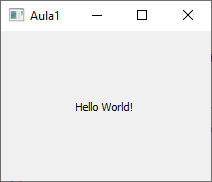
\includegraphics{janela}
    \caption{Janela Principal}
    \label{}
\end{figure}
\end{document}